%%% Copyright (C) 2018 Vincent Goulet
%%%
%%% Ce fichier fait partie du projet
%%% «Programmer avec R»
%%% https://gitlab.com/vigou3/programmer-avec-r
%%%
%%% Cette création est mise à disposition selon le contrat
%%% Attribution-Partage dans les mêmes conditions 4.0
%%% International de Creative Commons.
%%% https://creativecommons.org/licenses/by-sa/4.0/

%%%
%%% Page de titre
%%%

\begingroup
\TPGrid{3}{36}
\textblockorigin{0mm}{0mm}
\setlength{\parindent}{0mm}
\setlength{\imageheight}{29\TPVertModule}
\setlength{\banderougewidth}{2\TPHorizModule}
\setlength{\banderougeheight}{\TPVertModule}
\setlength{\bandeorwidth}{\TPHorizModule}
\setlength{\bandeorheight}{\banderougeheight}
\setlength{\logoheight}{2.5\TPVertModule}
\setlength{\gapwidth}{1.5pt}
\addtolength{\bandeorwidth}{-\gapwidth}
\addtolength{\imageheight}{-\gapwidth}
\setlength{\fboxrule}{3pt}
\setlength{\fboxsep}{0pt}

\def\titlefmt{%
  \sffamily\bfseries\fontsize{52}{52}\selectfont\thetitle}
\def\authorfmt{%
  \sffamily\mdseries\fontsize{30}{38}\selectfont\theauthor}
\def\affiliation{%
  \sffamily\mdseries\fontsize{22}{26}\selectfont
  Professeur titulaire \\
  École d'actuariat, Université Laval}
\def\edition{%
  \sffamily\mdseries\fontsize{22}{26}\selectfont
  Édition {\fullcaps\year}.\month}

%% bandeau identitaire
\begin{textblock*}{\paperwidth}[0,1](0mm,30\TPVertModule)
  \textcolor{rouge}{\rule{\banderougewidth}{\banderougeheight}}% % bande rouge
  \rule{\gapwidth}{0pt}%                                         % filet
  \textcolor{or}{\rule{\bandeorwidth}{\bandeorheight}}           % bande or
\end{textblock*}

%% logo UL
\begin{textblock*}{\TPHorizModule}(2\TPHorizModule,31\TPVertModule)
  \rule{\gapwidth}{0pt}%                                         % filet
  
\includegraphics[height=\logoheight,%
                   keepaspectratio=true]{ul_p}
\end{textblock*}

%% image de fond
\begin{textblock*}{\paperwidth}(0mm,0mm)
  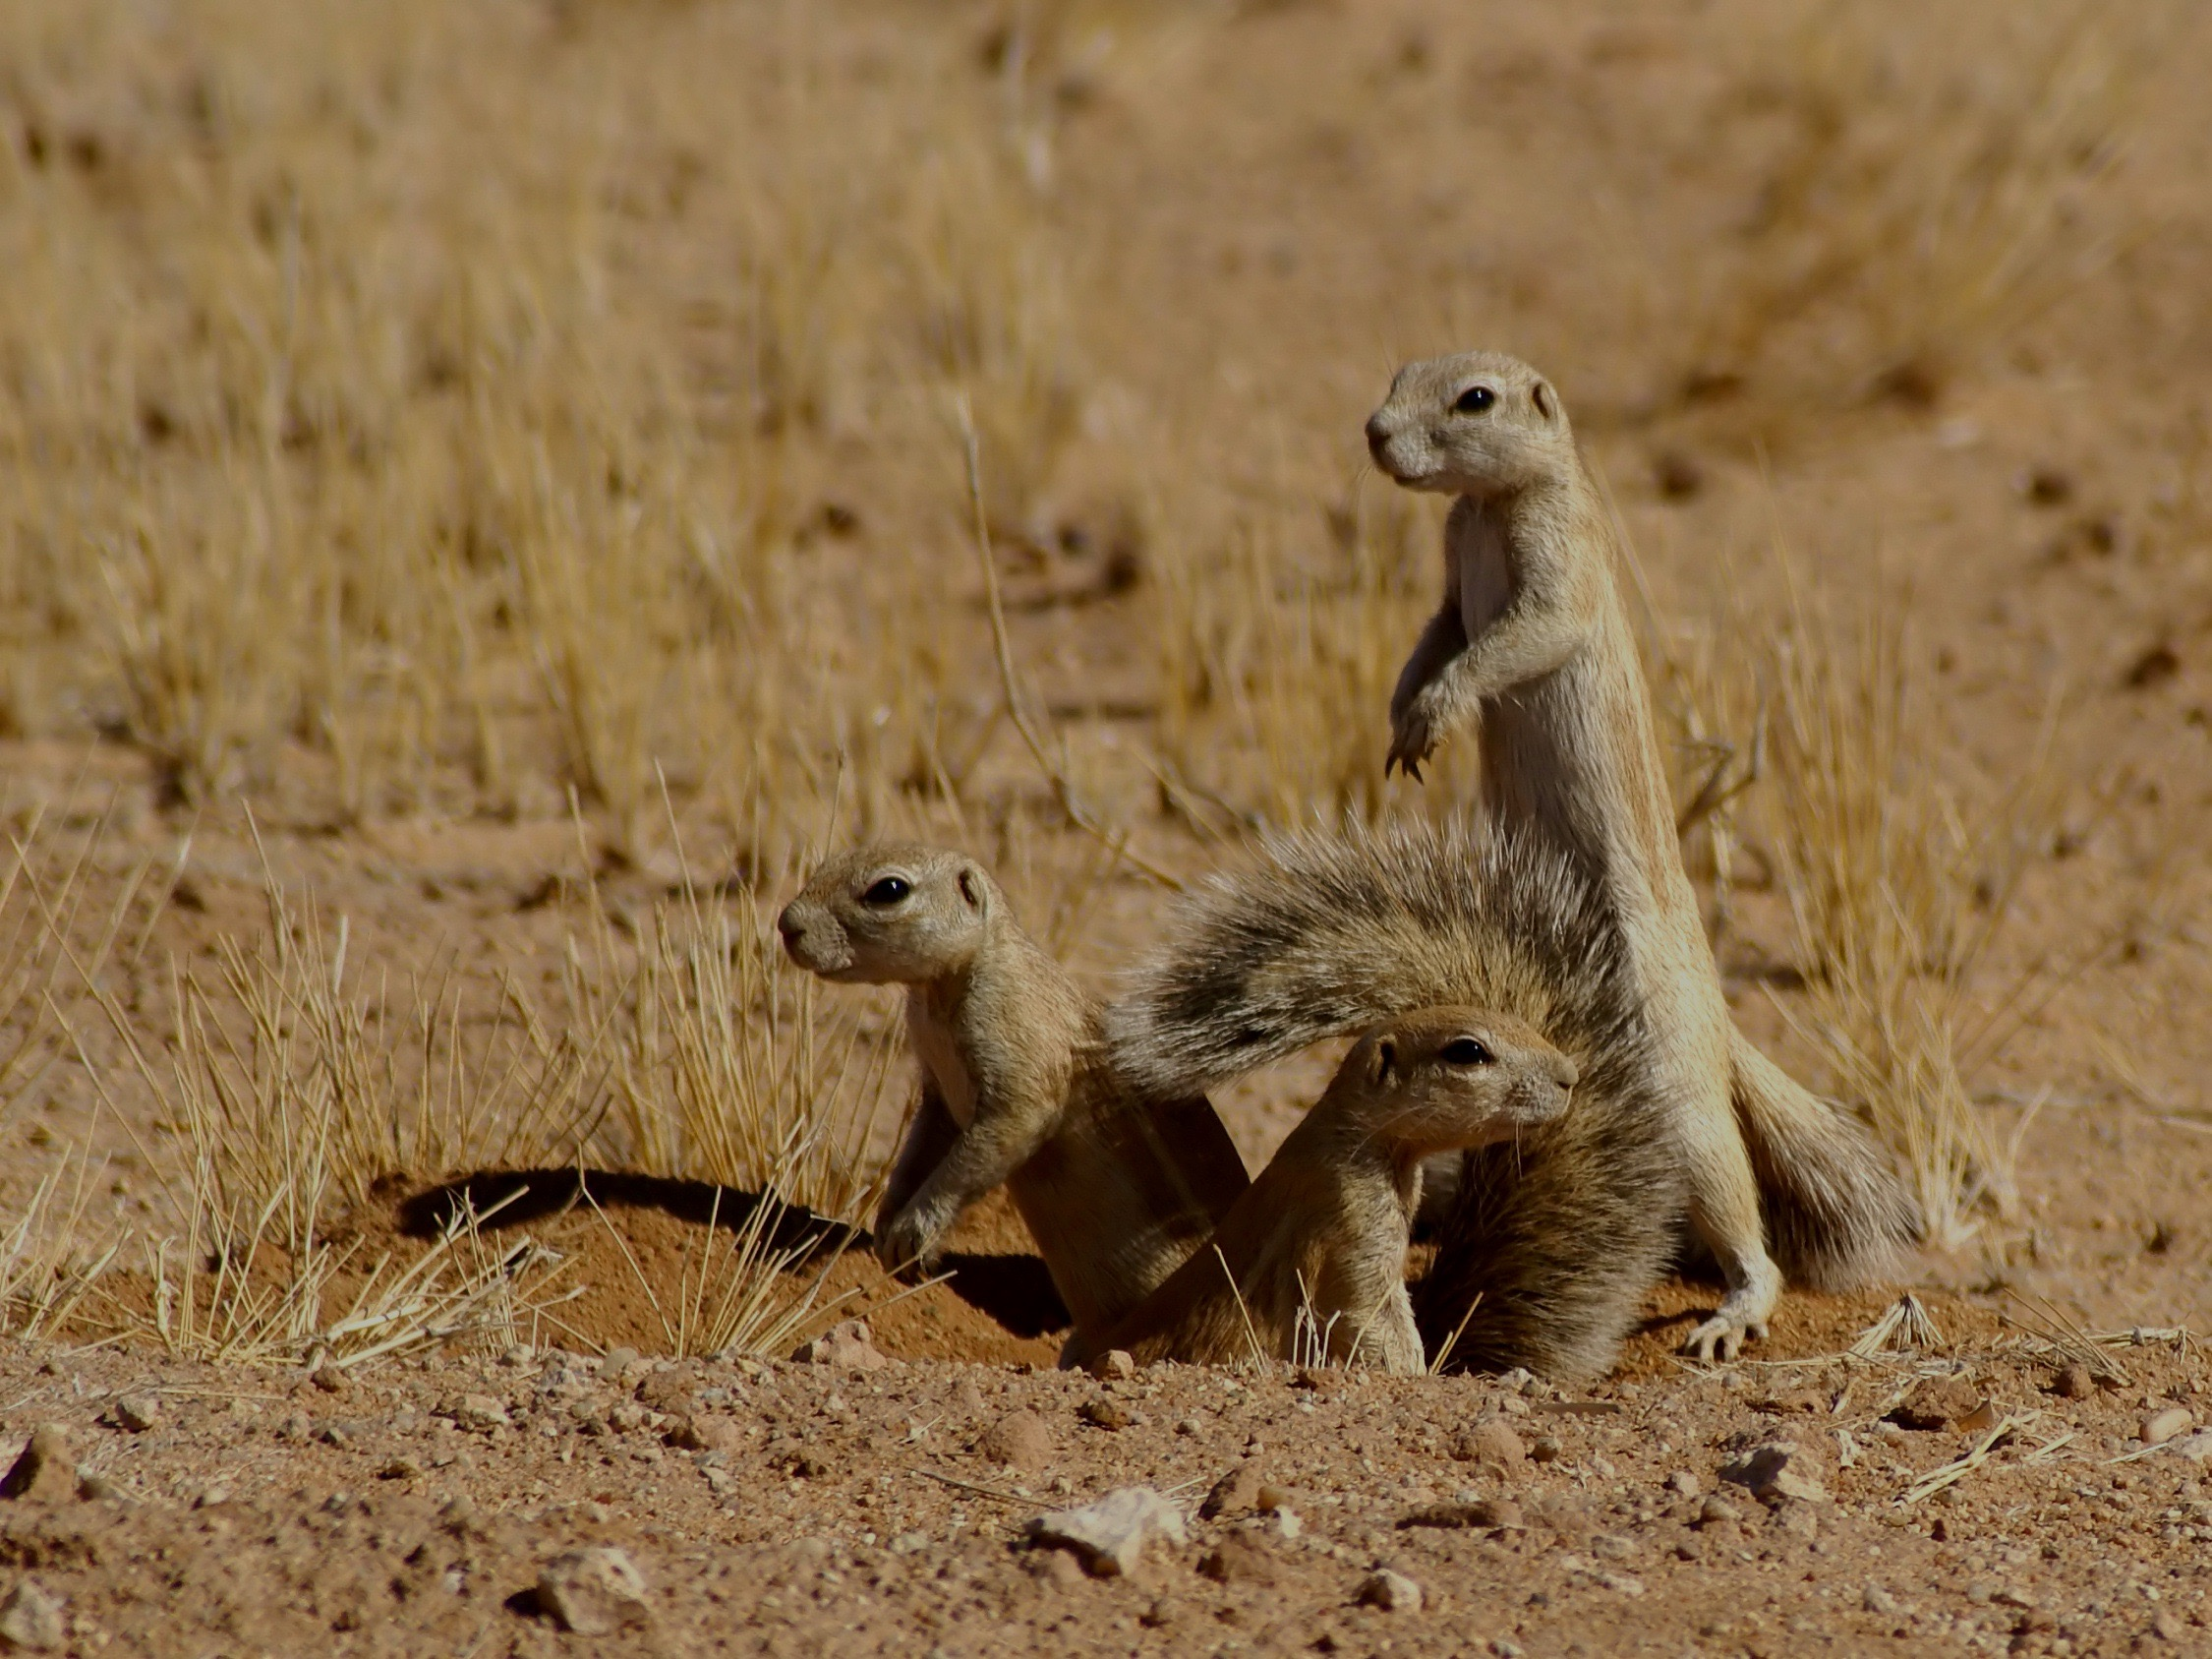
\includegraphics[height=\imageheight,%
                   width=\paperwidth,%
                   trim=555 185 251 0,clip]{Xerus_inauris_1}
\end{textblock*}

%% titre
\begin{textblock*}{\paperwidth}(0.3\TPHorizModule,3.1\TPVertModule)
  \pgfsetfillopacity{0.6}
  \fbox{\textcolor{white}{\rule{2.27\TPHorizModule}{2.9\TPVertModule}}}
  \pgfsetfillopacity{1}
\end{textblock*}
\begin{textblock*}{\paperwidth}(0.35\TPHorizModule,3.7\TPVertModule)
  \titlefmt
\end{textblock*}

%% auteur
\begin{textblock*}{\paperwidth}(0.3\TPHorizModule,6.6\TPVertModule)
  \pgfsetfillopacity{0.6}
  \fbox{\textcolor{white}{\rule{0.97\TPHorizModule}{2.0\TPVertModule}}}
  \pgfsetfillopacity{1}
\end{textblock*}
\begin{textblock*}{\paperwidth}(0.35\TPHorizModule,7.2\TPVertModule)
  \authorfmt
\end{textblock*}

\null\cleardoublepage

%%%
%%% Page frontispice
%%%

%% titre
\begin{textblock*}{\paperwidth}(0.35\TPHorizModule,3.7\TPVertModule)
  \titlefmt
\end{textblock*}

%% auteur
\begin{textblock*}{2\TPHorizModule}(0.35\TPHorizModule,7.2\TPVertModule)
  \authorfmt
\end{textblock*}

%% affiliation
\begin{textblock*}{2\TPHorizModule}(0.35\TPHorizModule,9.7\TPVertModule)
  \affiliation
\end{textblock*}

%% édition
\begin{textblock*}{1.7\TPHorizModule}(0.35\TPHorizModule,30\TPVertModule)
  \edition
\end{textblock*}
\endgroup

%%% Local Variables:
%%% mode: latex
%%% TeX-master: "programmer-avec-r"
%%% TeX-engine: xetex
%%% End:
